\documentclass[a4paper, 12pt]{report}

\usepackage{lmodern} % Police standard sous LaTeX : Latin
\usepackage[english]{babel} % Pour la langue anglaise
\usepackage[utf8]{inputenc} % Pour l'UTF-8
\usepackage[T1]{fontenc} % Pour les césures des caractères
\usepackage{graphicx}
\usepackage{subfig}
\usepackage{ragged2e}
\justifying

\renewcommand{\thesection}{\Alph{section}}

\title{Model of the spread of a disease in a population of mobile agents}
\author{NIDDAM Benjamin}
\date{\today}

\begin{document}
\begin{titlepage}
	\maketitle
\end{titlepage}

\newpage

\tableofcontents

\newpage
\section{Introduction}
The modeling of spatial segregation proposed in the 1970s by Thomas
C. Schelling made an impression because of the perverse effect she suggested: a strong
segregation could be the collective result of individual decisions that are not aimed at
such segregation. We would be dealing with an almost spontaneous phenomenon. The problem is
that such a conclusion outright contradicts the entropy principle. An exam
more attentive to the model makes it possible here to identify no less than four biases which condition the
results. We will study here the impacts that population density and the dissatisfaction rate can have on segregation.

\section{Model presentation}

Schelling's model is a model of spatial segregation. It takes the form of a matrix of n * n boxes.
Each cell is represented by an integer between -1, 0 and 1. Empty cells are represented by 0 while cells
occupied by an individual are represented by a -1 or 1. We therefore obtain a stylized representation of two populations which
share an urban area.

Initially, the agents are placed at random to simulate the mix of populations. We then add a rule of
movement of agents: they will change boxes if, in their immediate neighborhood, there is not at least "n"
agents of the same type as them. When an agent is not satisfied, we generate a random place among the empty cells and we
place the agent in this box; which frees up its old place. This operation is carried out until all the agents
are satisfied, or until the defined maximum time is reached. Under these conditions, we obtain groupings of
populations which appeared without being intentionally provoked.

\newpage

\begin{figure}[ht]

	\centering
	\subfloat{{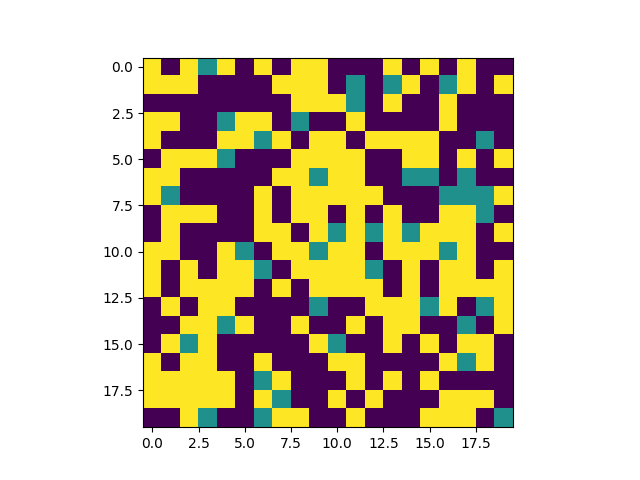
\includegraphics[width=6cm]{../resultats/worlds/Init/INS_0.6/initial_20.png} }}
	\centering
	\subfloat{{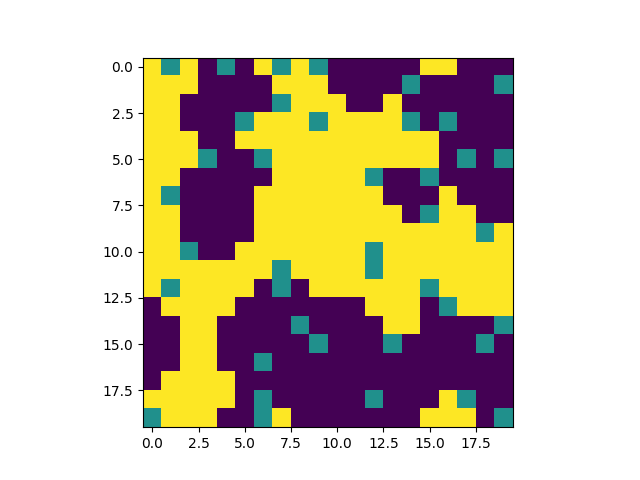
\includegraphics[width=6cm]{../resultats/worlds/Sorted/INS_0.6/sorted_20.png} }}
	\caption{Graphic representations of the initial and segregated populations with Schelling's model}

\end{figure}

\newpage

\section{Experiments, results}

With this model, we were able to study the effects of population density and insatisfaction rate on movements
agents.

\subsection{Population density}

As said, we have run several simulations with different population density values. In other words,
we wanted to study whether the number of free sites played a role in the separation of populations.

\vspace{0.7cm}

We varied the number of free cells from 15 to 24 and obtained the following results:

\begin{figure}[!h]
	\centering
	\subfloat[Initial state]{{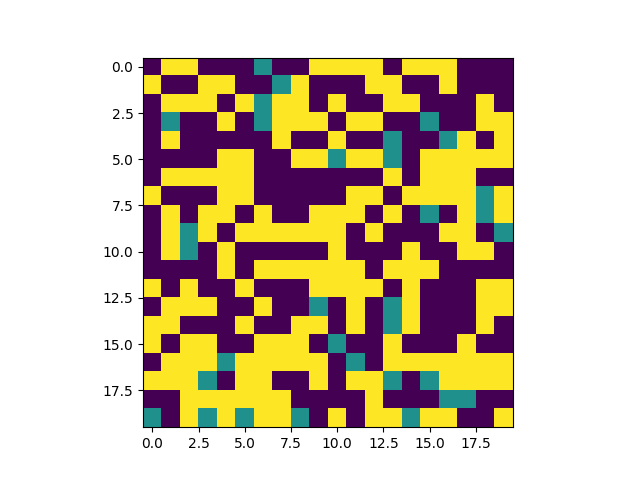
\includegraphics[width=6cm]{../resultats/worlds/Init/INS_0.5/initial_16.png} }}
	\subfloat[Population segregation after simulation]{{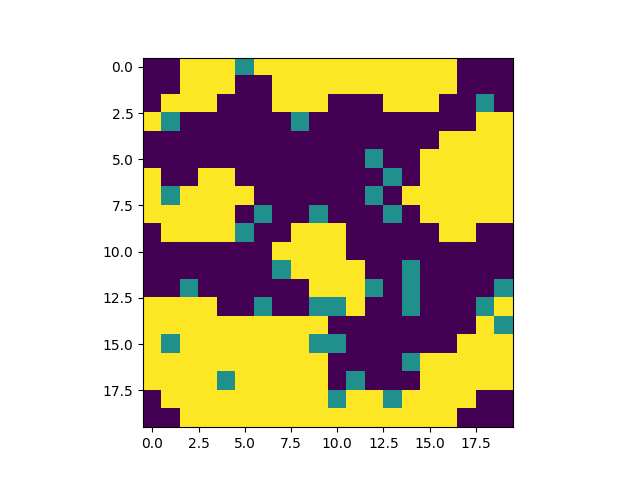
\includegraphics[width=6cm]{../resultats/worlds/Sorted/INS_0.5/sorted_16.png} }}
	\caption{Graphic representations of the initial and segregated states of Schelling's model with 16 free cells over 400 at an insatisfaction rate of 0.5}
\end{figure}

\begin{figure}[!h]
	\centering
	\subfloat[Initial state]{{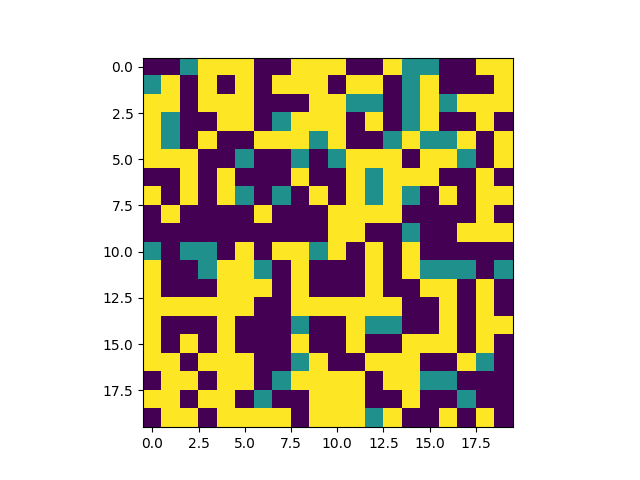
\includegraphics[width=6cm]{../resultats/worlds/Init/INS_0.5/initial_24.png} }}
	\subfloat[Population segregation after simulation]{{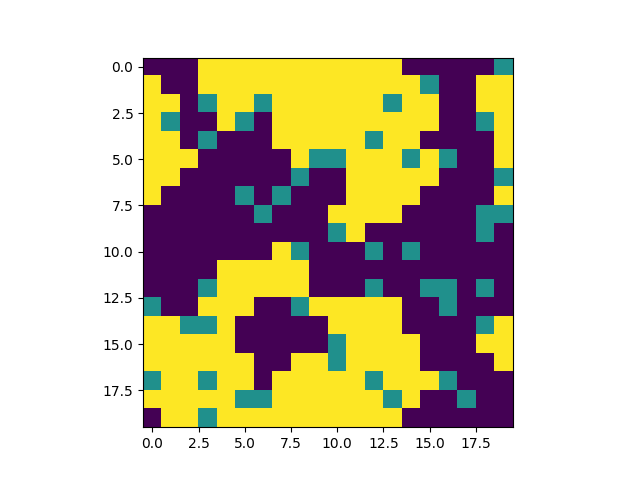
\includegraphics[width=6cm]{../resultats/worlds/Sorted/INS_0.5/sorted_24.png} }}
	\caption{Graphic representations of the initial and segregated states of Schelling's model with 24 free cells over 400 at an insatisfaction rate of 0.5}

\end{figure}

\newpage

It is observed that in both cases, the agents separated into two distinct groups according to their color. So we have
represented the time taken by our agents to arrive at a stable situation according to the population density.

\begin{figure}[!h]
	\centering
	% \subfloat{{\includegraphics[width=10cm]{../resultats/Curves/INS_evolution/} }}
	\caption{Graphic representations of the time spent by the agents to reach a stable state with a variable population density at an insatisfaction rate of 0.5}
\end{figure}

\newpage

We can see that the convergence time towards a stable state is longer as the population density increases. This is due to the decrease in the number of
free cells.

\subsection{Insatisfaction rate}

This time we have varied the dissatisfaction rate over a range of values from 0.1 to 0.9 with a step of 0.1. For these nine simulations, we obtained
very different results from each other:

\begin{figure}[!h]
	\centering
	\subfloat[Insatisfaction rate at 0.1]{{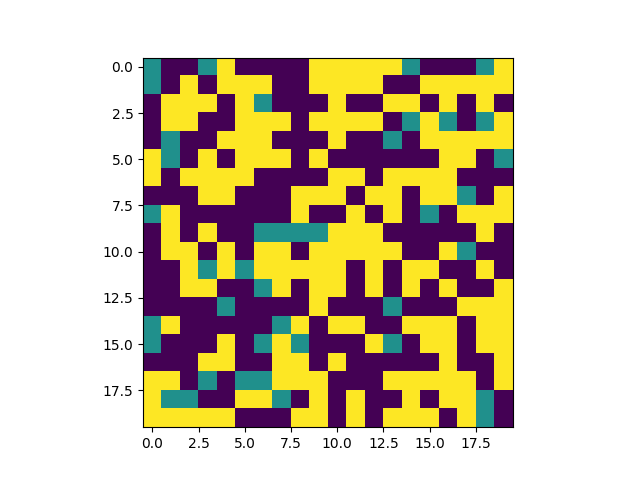
\includegraphics[width=6cm]{../resultats/worlds/Sorted/INS_0.1/sorted_20.png} }}
	\subfloat[Insatisfaction rate at 0.2]{{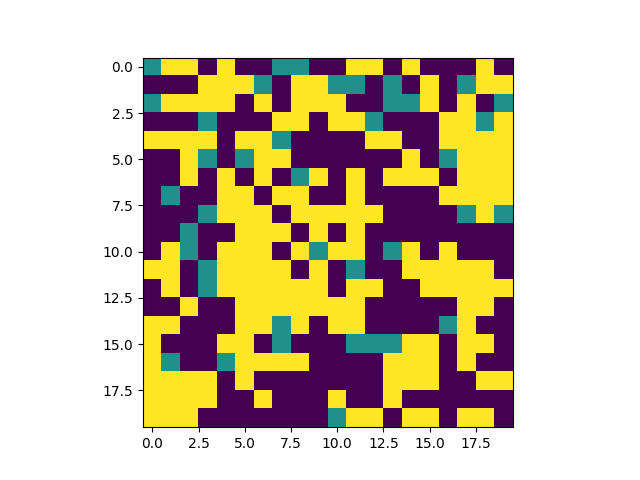
\includegraphics[width=6cm]{../resultats/worlds/Sorted/INS_0.2/sorted_20.png} }}
\end{figure}

\begin{figure}[!h]
	\centering
	\subfloat[Insatisfaction rate at 0.3]{{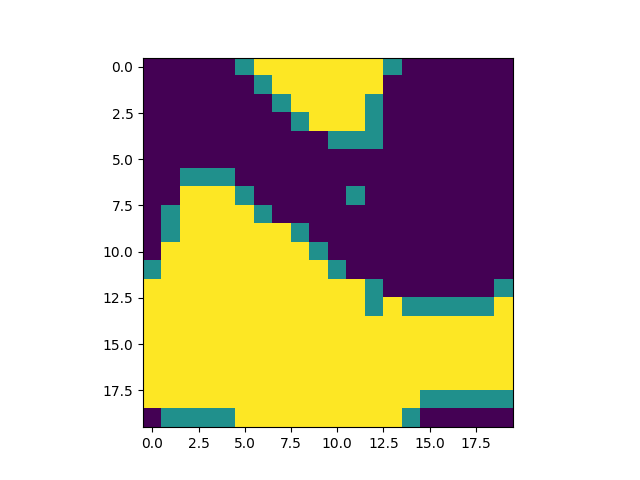
\includegraphics[width=6cm]{../resultats/worlds/Sorted/INS_0.3/sorted_20.png} }}
	\subfloat[Insatisfaction rate at 0.4]{{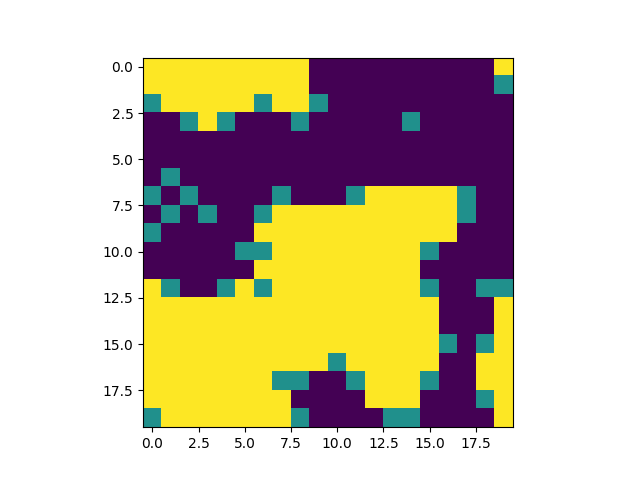
\includegraphics[width=6cm]{../resultats/worlds/Sorted/INS_0.4/sorted_20.png} }}
	\caption{Graphic representation of the organization of populations at the end of the simulations for a given dissatisfaction rate}
\end{figure}

\newpage

It is clear that the tendency of the population to separate regardless of the rate of dissatisfaction. With a threshold when the rate is 0.3 (1/3) from which this
segregation is becoming much more important. This rate, 1/3, is the rate found by Schelling for which it is impossible to obtain anything other than a state where
populations are separated. This is called the "law of thermodynamics".

\begin{figure}[!h]
	\centering
	\subfloat[Initial state]{{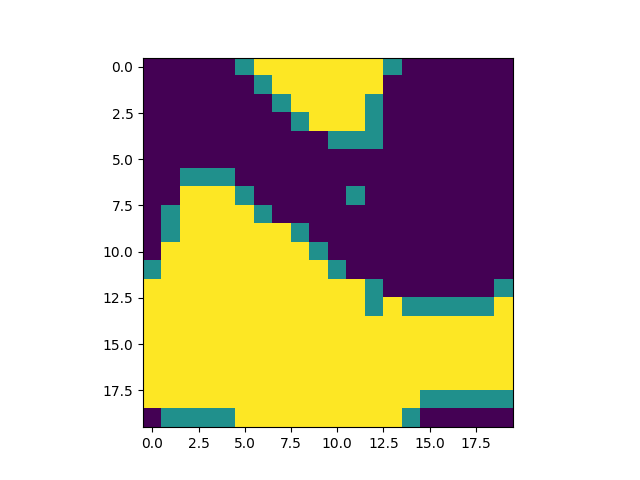
\includegraphics[width=6cm]{../resultats/worlds/Sorted/INS_0.3/sorted_20.png} }}
	\caption{Graphic representations of the initial and segregated states of Schelling's model with 24 free cells over 400 at an insatisfaction rate of 0.5}
\end{figure}

\section{Conclusion}
\end{document}

